
\documentclass[UTF8, onecolumn, a4paper]{article}
\usepackage{ctex}
\setlength{\parindent}{2em}
\usepackage{appendix}
\usepackage{geometry}
\usepackage{amsmath, amsthm}
\usepackage{multirow, multicol}
\usepackage{subfigure}
\usepackage{float}
\usepackage{graphicx}
\usepackage{lettrine}
\usepackage{authblk}
\usepackage{indentfirst}
\usepackage{xcolor, fontspec}%用于设置颜色
\usepackage[ruled,vlined]{algorithm2e}
\usepackage{listings}%用于显示代码
\usepackage[colorlinks,
linkcolor=black,
anchorcolor=blue,
citecolor=green
]{hyperref}
\usepackage{tikz}
\usetikzlibrary{trees}
\geometry{left=2.5cm,right=2.5cm,top=2.0cm,bottom=2.0cm}


\title{\textbf{点亮数字人生: 实验报告}}%———总标题
\author{刘泓尊\quad 2018011446\quad 计84}
%\affil{Department of Computer Science, Tsinghua University}

\begin{document}
\maketitle
\tableofcontents
\lstset{%代码块全局设置
	backgroundcolor=\color{red!3!green!3!blue!3},%代码块背景色为浅灰色
	rulesepcolor= \color{gray}, %代码块边框颜色
	breaklines=true,  %代码过长则换行
	numbers=left, %行号在左侧显示
	numberstyle= \small,%行号字体
	%keywordstyle= \color{red},%关键字颜色
	commentstyle=\color{gray}, %注释颜色
	frame=shadowbox,%用方框框住代码块
	xleftmargin=1em,
	xrightmargin=0em,
	tabsize=5,
	%rulesepcolor=\color{red!20!green!20!blue!20},  %阴影颜色
	keywordstyle={\color{blue!90!}\fontspec{Consolas Bold}},   %关键字颜色
	commentstyle={\color{blue!70!black}\fontspec{Consolas Italic}},   %注释颜色
	stringstyle=\color{orange!100!black}, %字符串颜色
	numberstyle=\color{purple}, %行号颜色
	%basicstyle=\ttfamily, %代码风格
	basicstyle=\fontspec{Consolas},
	showstringspaces=false,          % underline spaces within strings only  
	showtabs=false,
	captionpos=t, %文件标题位置
	flexiblecolumns
}
\vspace*{20}
\section{File Structure}
\tikzstyle{every node}=[draw=black,thick,anchor=west]
\tikzstyle{selected}=[draw=red,fill=red!30]
\tikzstyle{optional}=[dashed,fill=gray!50]
\begin{center}
	\begin{tikzpicture}
	[
	grow via three points={one child at (0.5,-0.7) and
		two children at (0.5,-0.7) and (0.5,-1.4)},
	edge from parent path={(\tikzparentnode.south)  |-(\tikzchildnode.west)}]
	\node {2018011446}
	child { node {lighten2.vhd} }
	child { node {decoder.vhd} }
	child { node {Waveform.vwf} }
	child { node {JieLabs录屏.mp4} }
	child { node {2018011446\_刘泓尊\_点亮数字人生.pdf} };
	\end{tikzpicture}
\end{center}

\clearpage
\section{实验目的}
\begin{enumerate}
	\item[(1)] 通过数码管点亮程序,熟悉VHDL语言,了解掌握硬件程序的编写规范
	\item[(2)] 掌握EDA软件的使用方法和工作流程
	\item[(3)] 进一步理解可编程芯片的工作原理
\end{enumerate}
\section{实验任务}
\paragraph*{}
设计一个数码管显示实验,要求七段数码管有规律地显示数列(奇数列,偶数列和自然数列),尽可能多地点亮数码管。要求实验中至少使用一个不带译码的数码管,充分利用实验平台上的接口和按键(CLK,RST)。
\paragraph*{}
本实验中,我使用1个不带译码的数码管显示自然数列(0 ~ F),2个带译码的数码管显示奇数列(1, 3, 5, 7, 9)和偶数列(0, 2, 4, 6, 8)。并进行了modelsim仿真和jielab实验平台仿真.

\section{代码解释及注释}
\subsection{4位2进制译码器}
基于模块化设计的思想,我首先编写了编码器(decoder)元件,将4位二进制数根据数码管的规则译码为7位二进制数,用于7段数码管的显示。之后在顶层实体中进行元件例化。代码如下:

\begin{lstlisting}[language={VHDL}, title={decoder.vhd}]
library ieee;
use ieee.std_logic_1164.all;
use ieee.std_logic_arith.all;
use ieee.std_logic_unsigned.all;

entity decoder is
	port(
		bit_4_vec: in std_logic_vector(3 downto 0);
		bit_7_vec: out std_logic_vector(6 downto 0)
	);
end decoder;

architecture bhv of decoder is begin
	process(bit_4_vec) begin
		case bit_4_vec is --译码处理
			when "0000" => bit_7_vec <= "1111110";
			when "0001" => bit_7_vec <= "0110000";
			when "0010" => bit_7_vec <= "1101101";
			when "0011" => bit_7_vec <= "1111001";
			when "0100" => bit_7_vec <= "0110011";
			when "0101" => bit_7_vec <= "1011011";
			when "0110" => bit_7_vec <= "1011111";
			when "0111" => bit_7_vec <= "1110000";
			when "1000" => bit_7_vec <= "1111111";
			when "1001" => bit_7_vec <= "1110011";
			when "1010" => bit_7_vec <= "1110111";
			when "1011" => bit_7_vec <= "0011111";
			when "1100" => bit_7_vec <= "1001110";
			when "1101" => bit_7_vec <= "0111101";
			when "1110" => bit_7_vec <= "1001111";
			when "1111" => bit_7_vec <= "1000111";
			when others => bit_7_vec <= "0000000"; --其他情况全灭
		end case;
	end process;
end bhv;
\end{lstlisting}
\subsection{三种数列的更新}
在顶层实体文件中,我设置了计数器count,每遇到一次时钟上升沿便+1,count每超过1,000,000时,重置count为0,之后将奇数列、偶数列、自然数列对应的std\_logic\_vector加1,实现数列的更新。这样处理,可以在1MHz的时钟周期下实现每1s更新一次数字。具体代码如下:
\begin{lstlisting}[language={VHDL}, title={lighten2.vhd}]
--点亮数字人生, 使用1个不带译码,2个带译码的数码管--
library ieee;
use ieee.std_logic_1164.all;
use ieee.std_logic_arith.all;
use ieee.std_logic_unsigned.all;

entity lighten2 is 
	port(
		clk: in std_logic; --控制时序变化
		rst: in std_logic; --重置
		display_4: out std_logic_vector(6 downto 0); --Without Decoder
		display_4_odd: out std_logic_vector(3 downto 0); --With Decoder
		display_4_even: out std_logic_vector(3 downto 0) --With Decoder
	);
end lighten2;

architecture bhv of lighten2 is
	component decoder --译码器例化
		port(
			bit_4_vec: in std_logic_vector(3 downto 0);
			bit_7_vec: out std_logic_vector(6 downto 0)
		);
	end component;
	signal display_4_odd_buf: std_logic_vector(3 downto 0) := "0001";--奇数
	signal display_4_even_buf: std_logic_vector(3 downto 0) := "0000";--偶数
	signal display_4_buf: std_logic_vector(3 downto 0) := "0000";--自然数
	signal count: integer := 0; --计数器
begin
	u1: decoder port map(bit_4_vec=>display_4_buf, bit_7_vec=>display_4);--译码
	display_4_even <= display_4_even_buf;--带译码器的直接输出
	display_4_odd <= display_4_odd_buf;  --带译码器的直接输出
	process(clk, rst) begin--时钟控制周期信号
		if rst='1' then --异步复位
			count <= 0;
			display_4_buf <= "0000";--reset
			display_4_even_buf <= "0000";
			display_4_odd_buf <= "0001";
		elsif clk'event and clk='1' then --处在上升沿看,也可以用rising_edge(clk)
			if count < 1_000_000 then --每1000000次上升,也就是当1MHz(1000ns)时钟频率时,1s更新1次(仿真的时候设为1, 即一次上升沿更新一次)
				count <= count + 1;
			else
				count <= 0;
				if display_4_buf = "1111" then
					display_4_buf <= "0000";--重置:F->0
				else
					display_4_buf <= display_4_buf + 1;--更新自然数
				end if;
				if display_4_even_buf = "1000" then
					display_4_even_buf <= "0000";--重置:8->0
				else
					display_4_even_buf <= display_4_even_buf + 2;--更新偶数
				end if;
				if display_4_odd_buf = "1001" then
					display_4_odd_buf <= "0001";--重置9->1
				else
					display_4_odd_buf <= display_4_odd_buf + 2;--更新奇数
				end if;
			end if;
		end if;
	end process;
end bhv;
\end{lstlisting}

\section{仿真结果}
使用Quartus的ModelSim进行仿真(根目录附"\textbf{Waveform.vwf}"文件),结果如下(仿真时代码的计数器更新间隔做了调整,以保证展示更多的数字).
可以看到,仿真结果与预期一致,每隔一定时间,三个数列分别以自然数列、奇数列、偶数列更新。
\begin{figure}[htb]
	\centering
	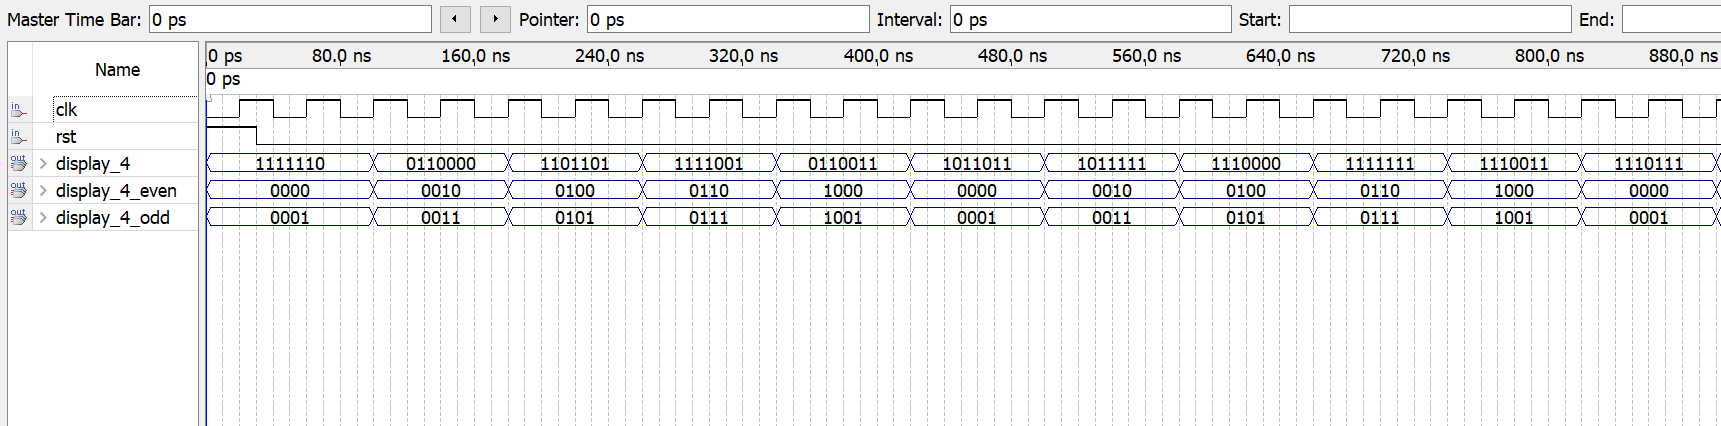
\includegraphics[width=1.0\textwidth]{simulation.png}
\end{figure}
\section{JieLab运行结果(附录屏)}
我将代码放在了JieLab实验平台上进行了验证,下面是运行时的截图,在根目录下有"\textbf{JieLabs录屏.mp4}",您可以更直观地检查我的实现效果,视频时长50s,详细展示了三种数列[自然数列(左)、奇数列(中)、偶数列(右)]的更新与复位(rst)操作.
\begin{figure}[htb]
	\centering
	\includegraphics[width=0.8\textwidth]{jielab.png}
\end{figure}
\section{实验总结}
\paragraph*{}
这是我第一次进行VHDL的编写,自己完成了QuartusII的安装、配置与VHDL的训练、仿真。我初步了解了VHDL的编写规范和语言特点,算是推开了"数字人生"的大门,也燃起了自己设计一些有趣的硬件的兴趣,。
\paragraph*{}
在此感谢老师、助教悉心准备的安装指南,这些视频节省了我很多时间!我还要感谢JieLab的推出,得益于此实验平台,我可以将我的代码进行直观的验证,免去了只进行仿真的"心虚"之感,引脚的分配与连接更是让我身临其境,收获良多。感谢实验平台开发者与老师、助教的悉心指导!

\end{document}